% 图 3.3 静电晶体场：(a) d_xy 与配体轨道错开（弱排斥）(b) d_{x2-y2} 正对配体（强重叠）
\documentclass[tikz,border=5pt]{standalone}
\usetikzlibrary{arrows.meta}
\usepackage{amsmath}
\usepackage{bm}
\usepackage{fontspec}
\setmainfont{Times New Roman}
\begin{document}
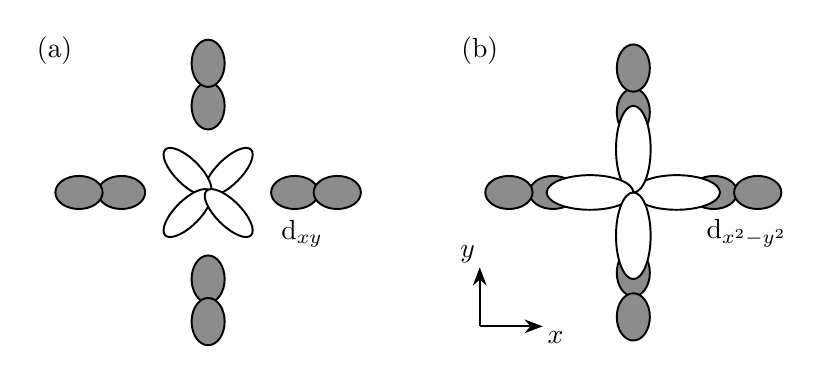
\begin{tikzpicture}[line width=0.8pt,>=Stealth]
% 配体 p 轨道（双瓣哑铃），#1 = 方位角
\newcommand{\ligand}[1]{
  \filldraw[fill=black!45,line width=0.7] (#1:1.10) ellipse [x radius=0.30,y radius=0.21,rotate=#1];
  \filldraw[fill=black!45,line width=0.7] (#1:1.64) ellipse [x radius=0.30,y radius=0.21,rotate=#1];
}
% ---------- (a) d_xy : 瓣沿对角方向，避开配体 ----------
\begin{scope}
\node at (-1.95,1.80) {(a)};
\foreach \a in {0,90,180,270}{\ligand{\a}}
% d_xy 四瓣（沿 45/135/225/315 度）
\foreach \a in {45,135,225,315}{
  \filldraw[fill=white,line width=0.7] (\a:0.37) ellipse [x radius=0.40,y radius=0.16,rotate=\a];
}
\node[anchor=west] at (0.80,-0.52) {$\mathrm{d}_{xy}$};
\end{scope}
% ---------- (b) d_x2-y2 : 瓣正对 ±x, ±y，与配体重叠 ----------
\begin{scope}[shift={(5.4,0)}]
\node at (-1.95,1.80) {(b)};
\foreach \a in {0,90,180,270}{
  \filldraw[fill=black!45,line width=0.7] (\a:1.02) ellipse [x radius=0.30,y radius=0.21,rotate=\a];
  \filldraw[fill=black!45,line width=0.7] (\a:1.58) ellipse [x radius=0.30,y radius=0.21,rotate=\a];
}
\foreach \a in {0,90,180,270}{
  \filldraw[fill=white,line width=0.7] (\a:0.55) ellipse [x radius=0.55,y radius=0.22,rotate=\a];
}
\node[anchor=west] at (0.80,-0.52) {$\mathrm{d}_{x^2-y^2}$};
% 小坐标系
\draw[->] (-1.95,-1.70) -- (-1.15,-1.70) node[below right=-2pt]{$x$};
\draw[->] (-1.95,-1.70) -- (-1.95,-0.95) node[above left=-2pt]{$y$};
\end{scope}
\end{tikzpicture}
\end{document}
